\documentclass[tikz]{standalone}

\usepackage{pgfplots}
\pgfplotsset{compat=1.16}

\begin{document}
    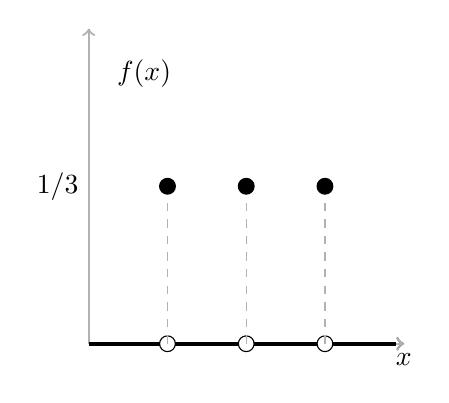
\begin{tikzpicture}
        \draw[step=2.5cm,gray,very thin] (0,0) grid (1,1);
        % Ejes
        \draw[thick,->] (0,0) -- (4,0) node[below, xshift=0pt]{$x$};
        \draw[thick,->, gray!60!white] (0,0) -- (4,0);
        \draw[thick] (0,0) -- (0,2) node[anchor=east] {$1/3$};
        \draw[thick] (0,0) -- (0,4) node[above, xshift=20pt, yshift=-25pt]{$f(x)$};
        \draw[thick,->, gray!60!white] (0,0) -- (0,4);
        % f(x)
        \draw[ultra thick] (0,0) -- (3.9,0);
        \foreach \x in {1,...,3}{
            \draw[fill=white] (\x,0) circle (0.1);
            \draw[dashed, gray!60!white] (\x,0) -- (\x,2);
            \draw[fill=black] (\x,2) circle (0.1);
        }
    \end{tikzpicture}
    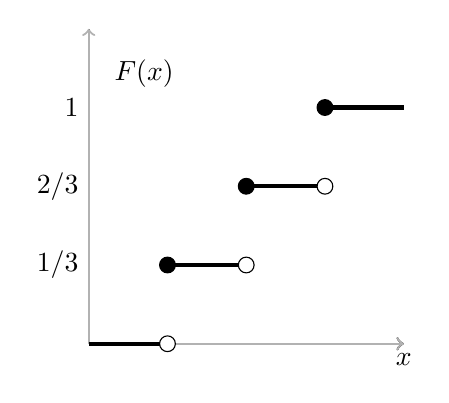
\begin{tikzpicture}
        \draw[step=2.5cm,gray,very thin] (0,0) grid (1,1);
        % Ejes y Leyendas
        \draw[thick,->] (0,0) -- (4,0) node[below, xshift=0pt]{$x$};
        \draw[thick,->, gray!60!white] (0,0) -- (4,0);
        \draw[thick] (0,0) -- (0,3) node[anchor=east] {$1$};
        \draw[thick] (0,0) -- (0,2) node[anchor=east] {$2/3$};
        \draw[thick] (0,0) -- (0,1) node[anchor=east] {$1/3$};
        \draw[thick] (0,0) -- (0,4) node[above, xshift=20pt, yshift=-25pt]{$F(x)$};
        \draw[thick,->, gray!60!white] (0,0) -- (0,4);
        % F(x)
        \draw[ultra thick] (0,0) -- (1,0);
        \draw[ultra thick] (1,1) -- (2,1);
        \draw[ultra thick] (2,2) -- (3,2);
        \draw[ultra thick] (3,3) -- (4,3);
        \foreach \x in {1,...,3}{
            \draw[fill=black] (\x,\x) circle (0.1);
            \draw[fill=white] (\x,\x-1) circle (0.1);
        }
    \end{tikzpicture}

    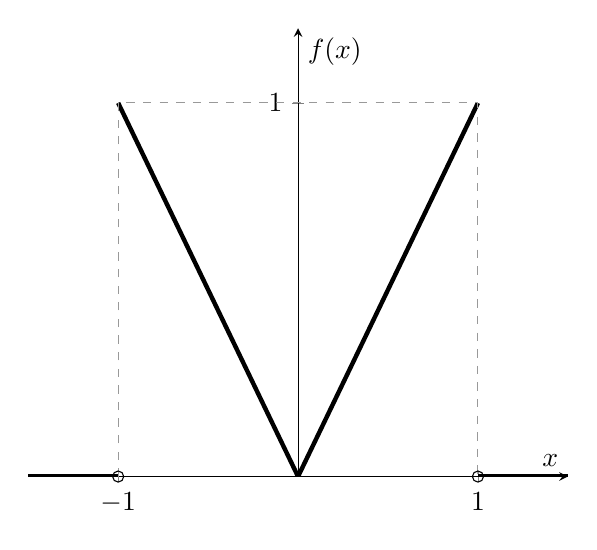
\begin{tikzpicture}
        % F(x)
        \begin{axis}[axis lines = center, xlabel = $x$, ylabel = {$f(x)$},ymax=1.2,ytick={1},xtick={-1,1}]
            \addplot[domain=-1.5:-1, samples=10,color=black, ultra thick]{0};
            \addplot[domain=-1:0, samples=10,color=black, ultra thick]{-x};
            \addplot[domain=0:1, samples=10,color=black, ultra thick]{x};
            \addplot[domain=1:1.5, samples=10,color=black, ultra thick]{0};
            \addplot[color=gray!80!white, style=dashed] coordinates{(-1,0)(-1,1)(1,1)(1,0)};
            \addplot[fill=white,mark=o] coordinates{(1,0)};
            \addplot[fill=white,mark=o] coordinates{(-1,0)};
        \end{axis}
    \end{tikzpicture}
    \begin{tikzpicture}
        % F(x)
        \begin{axis}[axis lines = center, xlabel = $x$, ylabel = {$F(x)$},ymax=1.2,ytick={1},xtick={-1,1}]
            \addplot[domain=-1.5:-1, samples=100,color=black, ultra thick]{0};
            \addplot[domain=-1:0, samples=100,color=black, ultra thick]{(1-x^2)/2};
            \addplot[domain=0:1, samples=100,color=black, ultra thick]{(1+x^2)/2};
            \addplot[domain=1:1.5, samples=100,color=black, ultra thick]{1};
            \addplot[color=gray!80!white, style=dashed] coordinates{(1,0)(1,1)};
            \addplot[color=gray!80!white, style=dashed] coordinates{(0,1)(1,1)};
        \end{axis}
    \end{tikzpicture}
\end{document}